%%%%%%%%%%%%%%%%%%%%%%%%%%%%%%%%%%%%%%%%%
% Short Sectioned Assignment
% LaTeX Template
% Version 1.0 (5/5/12)
%
% This template has been downloaded from:
% http://www.LaTeXTemplates.com
%
% Original author:
% Frits Wenneker (http://www.howtotex.com)
%
% License:
% CC BY-NC-SA 3.0 (http://creativecommons.org/licenses/by-nc-sa/3.0/)
%
%%%%%%%%%%%%%%%%%%%%%%%%%%%%%%%%%%%%%%%%%

%----------------------------------------------------------------------------------------
%	PACKAGES AND OTHER DOCUMENT CONFIGURATIONS
%----------------------------------------------------------------------------------------

\documentclass[paper=a4, fontsize=11pt]{scrartcl} % A4 paper and 11pt font size

\usepackage{comment}
\usepackage[T1]{fontenc} % Use 8-bit encoding that has 256 glyphs
\usepackage{fourier} % Use the Adobe Utopia font for the document - comment this line to return to the LaTeX default
\usepackage[english]{babel} % English language/hyphenation
\usepackage{amsmath,amsfonts,amsthm} % Math packages
\usepackage{listings}

\usepackage{lipsum} % Used for inserting dummy 'Lorem ipsum' text into the template
\usepackage{graphicx}

\usepackage{minted} % Used for Code Highlight

\usepackage{sectsty} % Allows customizing section commands
\allsectionsfont{\centering \normalfont\scshape} % Make all sections centered, the default font and small caps

\usepackage{fancyhdr} % Custom headers and footers
\pagestyle{fancyplain} % Makes all pages in the document conform to the custom headers and footers
\fancyhead{} % No page header - if you want one, create it in the same way as the footers below
\fancyfoot[L]{} % Empty left footer
\fancyfoot[C]{} % Empty center footer
\fancyfoot[R]{\thepage} % Page numbering for right footer
\renewcommand{\headrulewidth}{0pt} % Remove header underlines
\renewcommand{\footrulewidth}{0pt} % Remove footer underlines
\setlength{\headheight}{13.6pt} % Customize the height of the header

\numberwithin{equation}{section} % Number equations within sections (i.e. 1.1, 1.2, 2.1, 2.2 instead of 1, 2, 3, 4)
\numberwithin{figure}{section} % Number figures within sections (i.e. 1.1, 1.2, 2.1, 2.2 instead of 1, 2, 3, 4)
\numberwithin{table}{section} % Number tables within sections (i.e. 1.1, 1.2, 2.1, 2.2 instead of 1, 2, 3, 4)

\setlength\parindent{0pt} % Removes all indentation from paragraphs - comment this line for an assignment with lots of text

%----------------------------------------------------------------------------------------
%	TITLE SECTION
%----------------------------------------------------------------------------------------

\newcommand{\horrule}[1]{\rule{\linewidth}{#1}} % Create horizontal rule command with 1 argument of height

\title{	
\normalfont \normalsize 
\textsc{La Sapienza University of Rome. Department of Computer, Control, and Management Engineering} \\ [25pt] % Your university, school and/or department name(s)
\horrule{0.5pt} \\[0.4cm] % Thin top horizontal rule
\huge Interactive Graphics Final Project \\ % The assignment title
\horrule{2pt} \\[0.5cm] % Thick bottom horizontal rule
}

\author{Jean Pierre Richa, Simone Faricelli} % Your name

\date{\normalsize\today} % Today's date or a custom date

\begin{document}
\[%%%%%%%%%%%%%%%%%%%%%%%%%%%%%%%%%%%%%%%%%
% Short Sectioned Assignment
% LaTeX Template
% Version 1.0 (5/5/12)
%
% This template has been downloaded from:
% http://www.LaTeXTemplates.com
%
% Original author:
% Frits Wenneker (http://www.howtotex.com)
%
% License:
% CC BY-NC-SA 3.0 (http://creativecommons.org/licenses/by-nc-sa/3.0/)
%
%%%%%%%%%%%%%%%%%%%%%%%%%%%%%%%%%%%%%%%%%

%----------------------------------------------------------------------------------------
%	PACKAGES AND OTHER DOCUMENT CONFIGURATIONS
%----------------------------------------------------------------------------------------

\documentclass[paper=a4, fontsize=11pt]{scrartcl} % A4 paper and 11pt font size

\usepackage{comment}
\usepackage[T1]{fontenc} % Use 8-bit encoding that has 256 glyphs
\usepackage{fourier} % Use the Adobe Utopia font for the document - comment this line to return to the LaTeX default
\usepackage[english]{babel} % English language/hyphenation
\usepackage{amsmath,amsfonts,amsthm} % Math packages
\usepackage{listings}

\usepackage{lipsum} % Used for inserting dummy 'Lorem ipsum' text into the template
\usepackage{graphicx}

\usepackage{minted} % Used for Code Highlight

\usepackage{sectsty} % Allows customizing section commands
\allsectionsfont{\centering \normalfont\scshape} % Make all sections centered, the default font and small caps

\usepackage{fancyhdr} % Custom headers and footers
\pagestyle{fancyplain} % Makes all pages in the document conform to the custom headers and footers
\fancyhead{} % No page header - if you want one, create it in the same way as the footers below
\fancyfoot[L]{} % Empty left footer
\fancyfoot[C]{} % Empty center footer
\fancyfoot[R]{\thepage} % Page numbering for right footer
\renewcommand{\headrulewidth}{0pt} % Remove header underlines
\renewcommand{\footrulewidth}{0pt} % Remove footer underlines
\setlength{\headheight}{13.6pt} % Customize the height of the header

\numberwithin{equation}{section} % Number equations within sections (i.e. 1.1, 1.2, 2.1, 2.2 instead of 1, 2, 3, 4)
\numberwithin{figure}{section} % Number figures within sections (i.e. 1.1, 1.2, 2.1, 2.2 instead of 1, 2, 3, 4)
\numberwithin{table}{section} % Number tables within sections (i.e. 1.1, 1.2, 2.1, 2.2 instead of 1, 2, 3, 4)

\setlength\parindent{0pt} % Removes all indentation from paragraphs - comment this line for an assignment with lots of text

%----------------------------------------------------------------------------------------
%	TITLE SECTION
%----------------------------------------------------------------------------------------

\newcommand{\horrule}[1]{\rule{\linewidth}{#1}} % Create horizontal rule command with 1 argument of height

\title{	
\normalfont \normalsize 
\textsc{La Sapienza University of Rome. Department of Computer, Control, and Management Engineering} \\ [25pt] % Your university, school and/or department name(s)
\horrule{0.5pt} \\[0.4cm] % Thin top horizontal rule
\huge Interactive Graphics Final Project \\ % The assignment title
\horrule{2pt} \\[0.5cm] % Thick bottom horizontal rule
}

\author{Jean Pierre Richa, Simone Faricelli} % Your name

\date{\normalsize\today} % Today's date or a custom date

\begin{document}
\maketitle % Print the title
%----------------------------------------------------------------------------------------
%	PROBLEM 1
%----------------------------------------------------------------------------------------
\section{Introduction}

The project is about creating a game we named FishIt see figure \ref{world}, which is an interactive game made as close to reality as possible, it simulates a fisherman driving a boat inside a world consisting of everything that we can find in a real world fishing environment, such as the sky, sun, light-house, boat, rod, water, and fishes. The aim from the game is trying to catch as much fishes as possible. Each fish caught increases the total score by 1. \par We used rigid 3D objects, which we later animated using javascript such as the boat, and the rod, which can both be controlled by the user using the keyboard, and the fishes, which move randomly in the water. Furthermore, we included a human model hierarchical structure, which we are going to see in details when we discuss the implementation. The fishes move randomly and when the rod is thrown in the water, we wait for the bait to collide with a fish and give the user a counter specifying the time within which he should pull the rod to gain points, otherwise the fish will escape and he will not gain a new point.

\begin{figure}
\centering
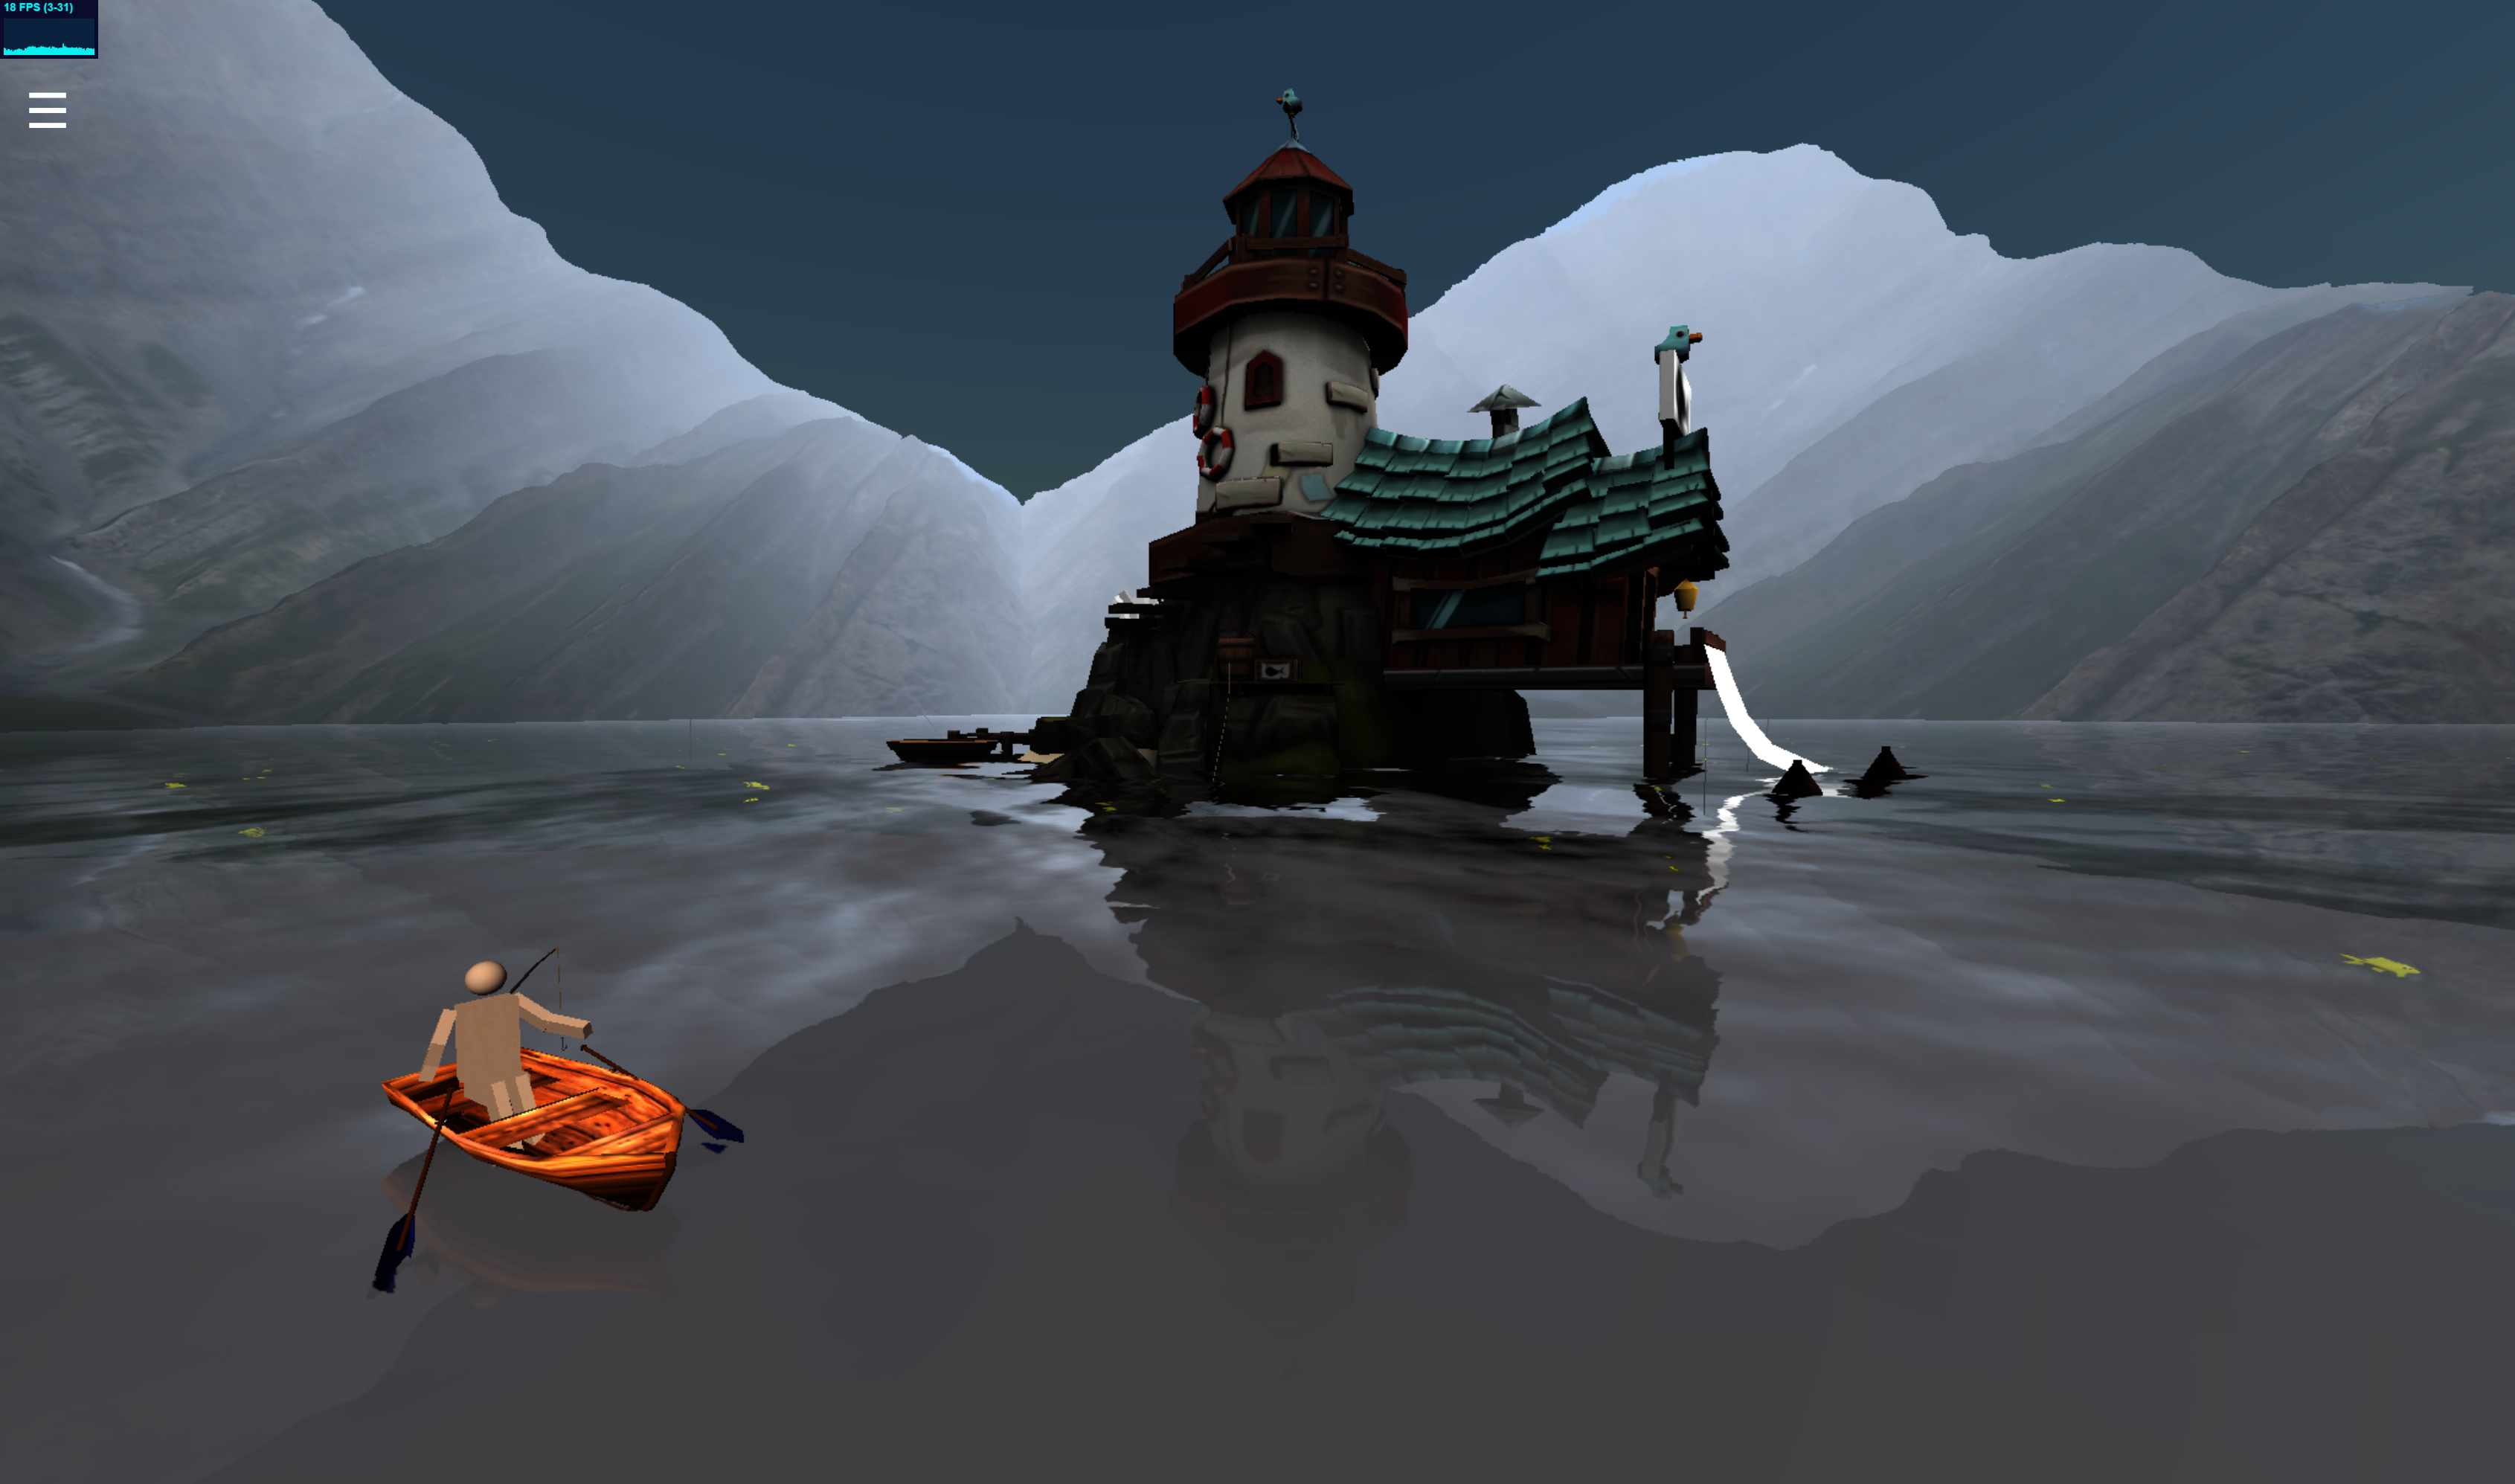
\includegraphics[width=15cm, height=6cm]{images/entire_scene.png}
\caption{Top view for the whole environment.}
\label{world}
\end{figure}

\newpage

%------------------------------------------------

%\subsection{Heading on level 2 (subsection)}
\section{Implementation}

In order to have a clear view about the implementation, this section will be split into several part, where each part will hold details about the implementation of each object. The areas that will be discussed in the following subsections are: the creation of each object, the placement in the environment, whether or not the object is controllable and how it is controllable, and other details specific to each object.

\subsection{Sky}

The first object to consider in this project is the sky, because we need the environment to look realistic. The sky is nothing but a \textit{Cube}, enlightened in a certain way and scaled by a value big enough to make it look continuous from the inside (See Figure \ref{external}). After that, the turbidity, luminance, and other characteristics were specified for the sky to fit this specific environment. The sky is clear and fixed, and cannot be controlled by the user. Finally, the above-mentioned characteristics were chosen to make the daytime look like if it's near the sunset. 
\begin{figure}
\centering
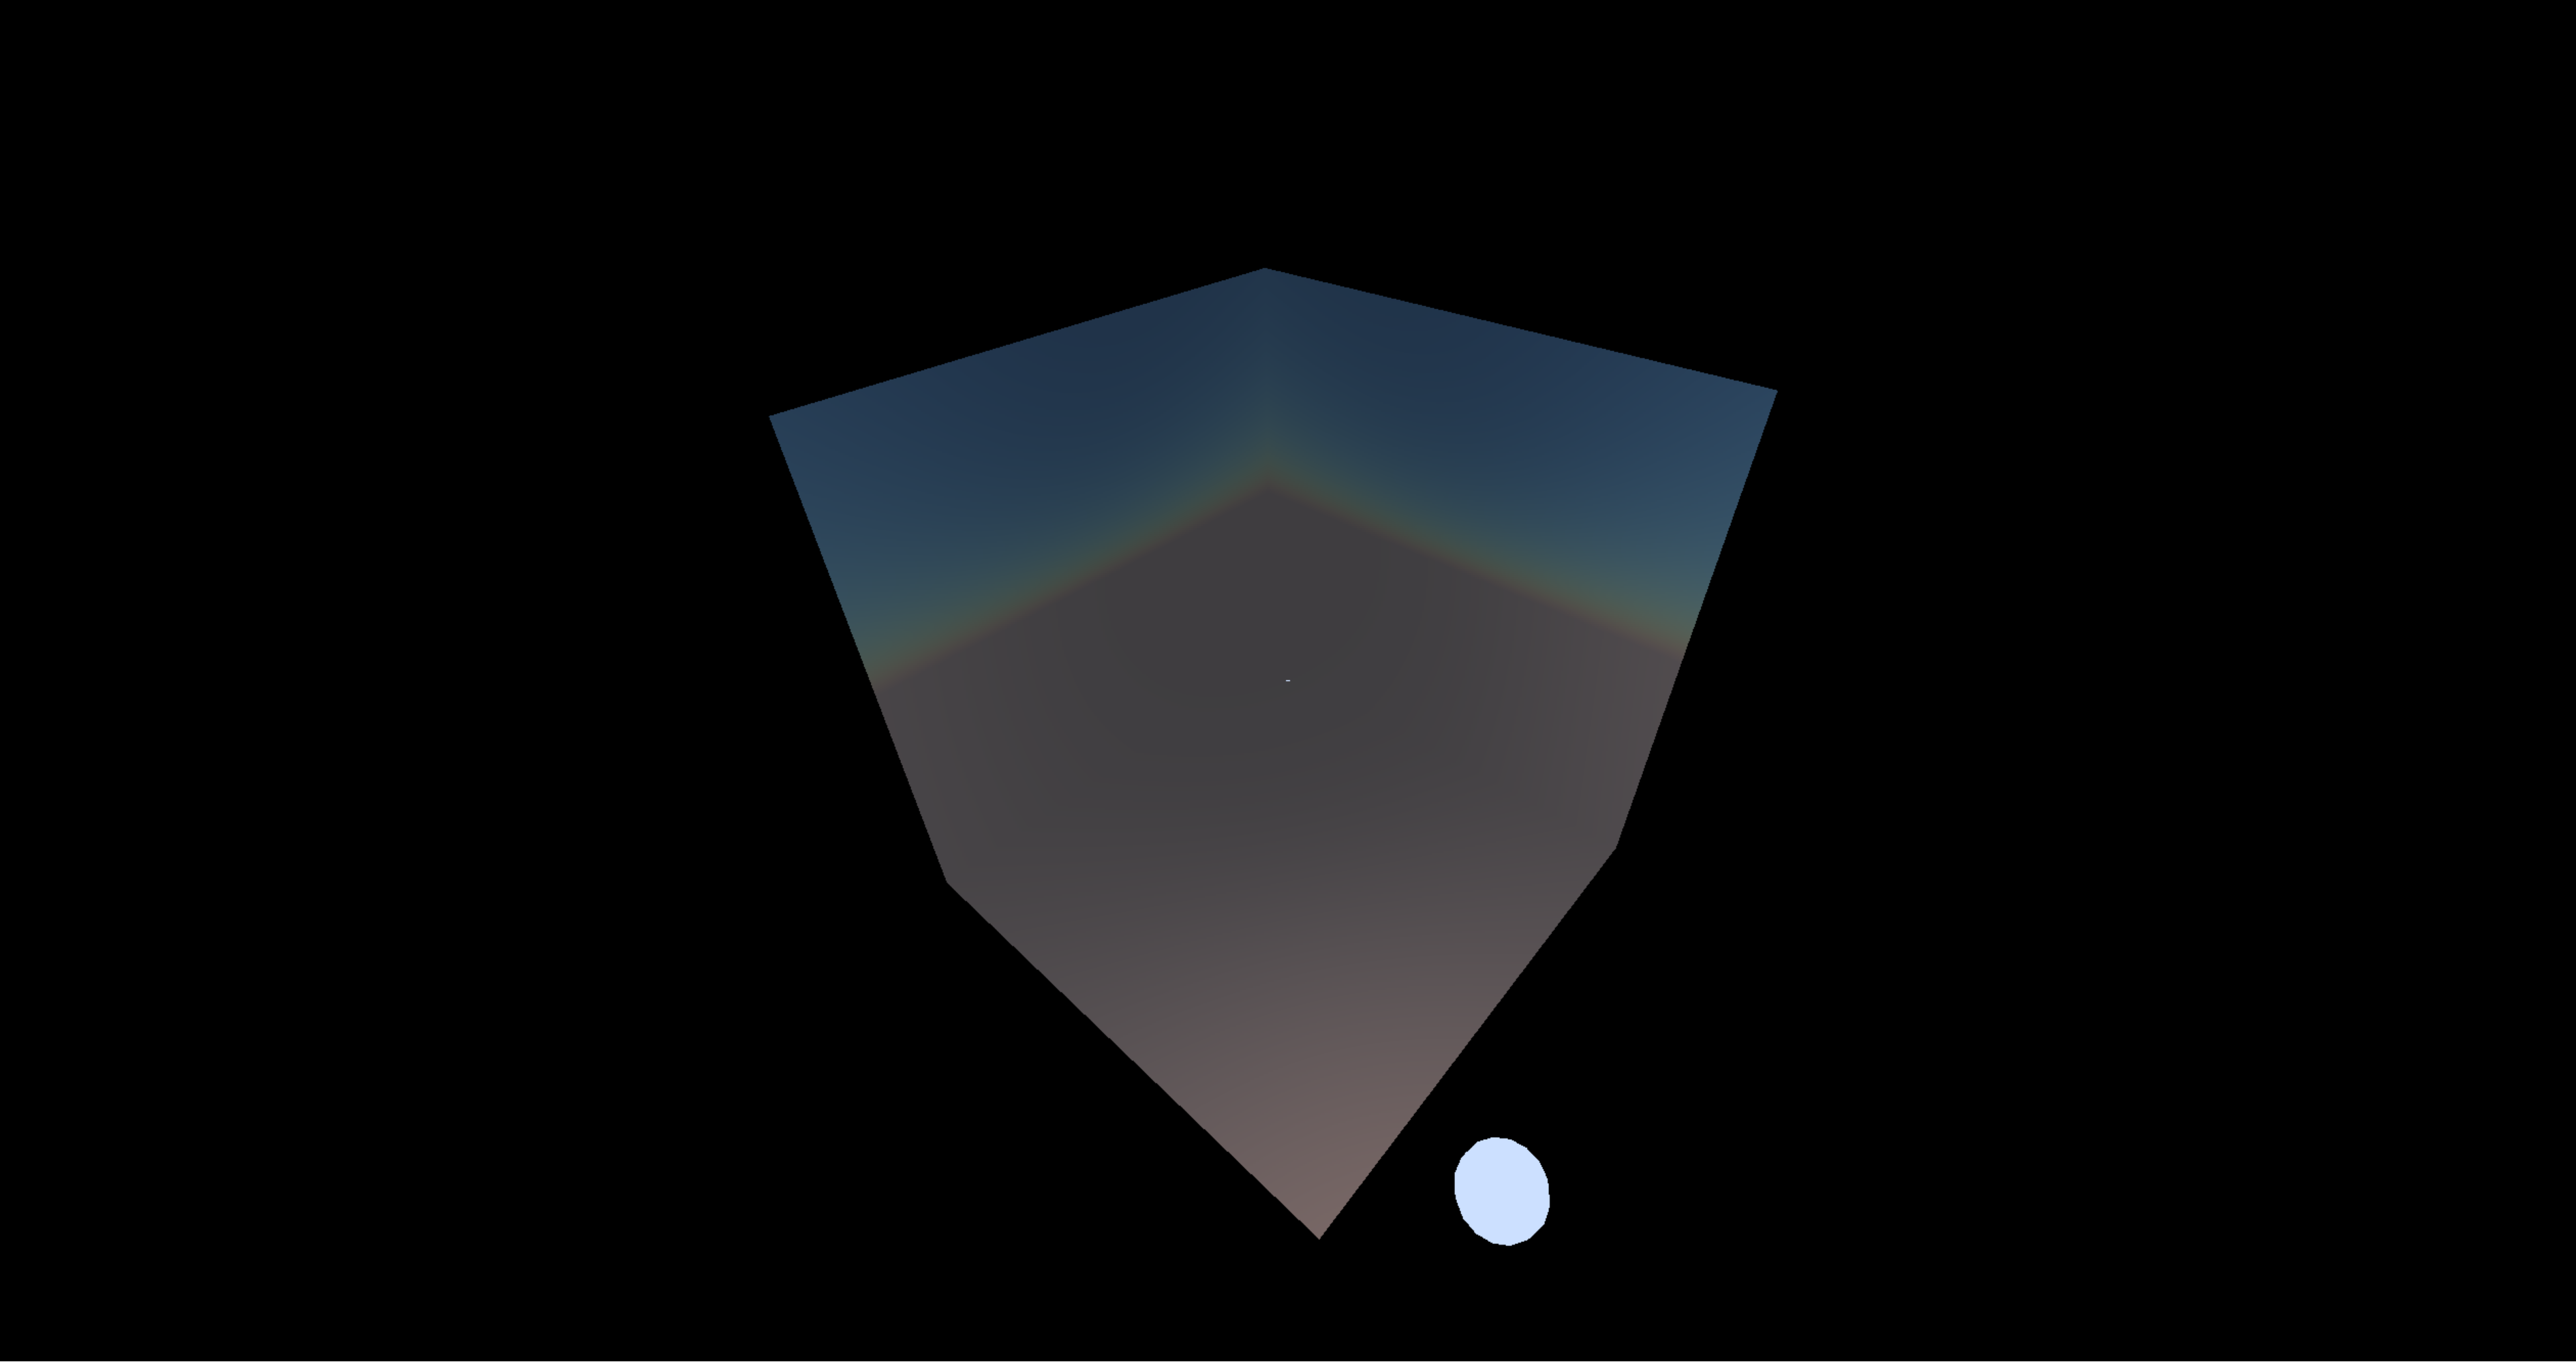
\includegraphics[width=15cm, height=6cm]{images/skyBox&sunSphere.png}
\caption{External view of the Sky Box and the Sun Sphere.}
\label{external}
\end{figure}

\newpage

\subsection{Sun and Light}

An important part of this project is the simulation of the sun as a light source. In order to have it, as for the sky, we added to the environment a huge \textit{Sphere}, positioning it really far away from the center of the scene to make it as realistic as possible.  After that, two light sources were added. The first one is a \textit{Directional Light}, which better simulates the sunlight when positioned in the same place of the sun sphere and directed at the scene, while the second one is an \textit{Ambient Light} in order to simulate the diffuse light all over the scene, created by the refraction of the sun light through the atmosphere. For better visualization check figure \ref{sun}. Moreover, another important issue to deal with when it comes to using lights in a scene is shadowing, so \textit{castShadow} function for the light was set to true in order to get the objects in the environment rendered into the shadow map.  \textbf{See also the Code section}.

\begin{figure}[!ht]
\centering
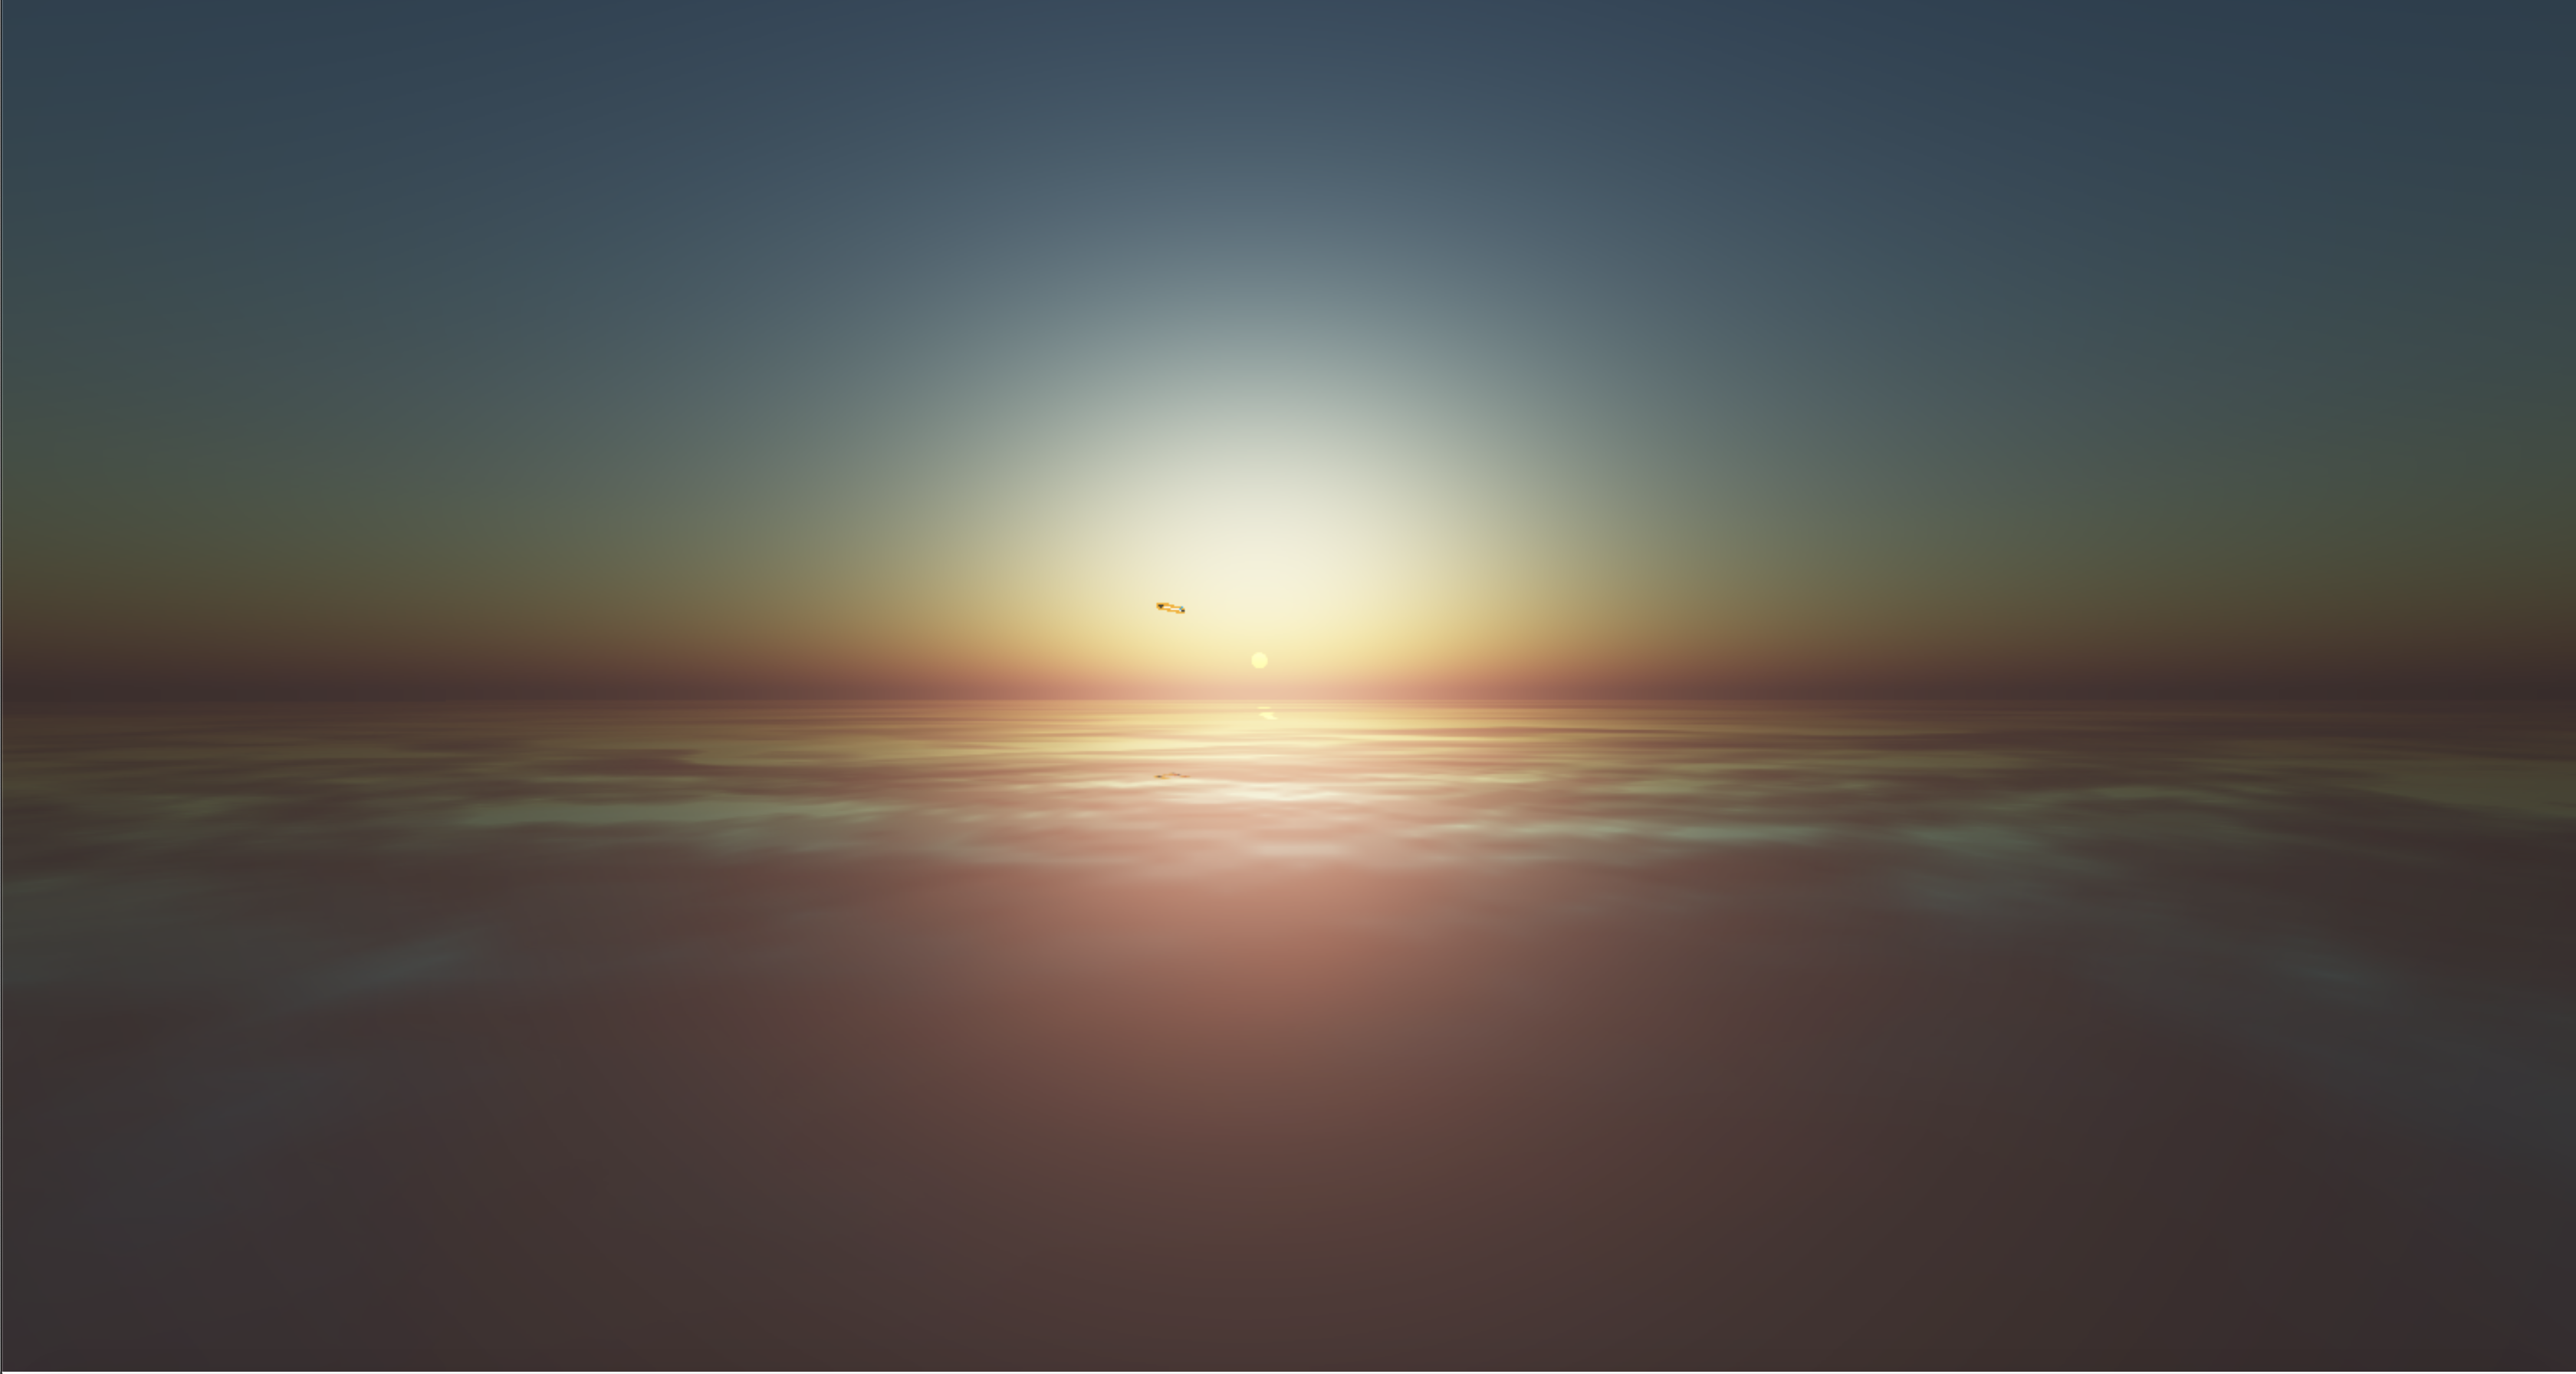
\includegraphics[width=15cm, height=6cm]{images/sun.png}
\caption{The sun viewed from the lake.}
\label{sun}
\end{figure}

\begin{minted}{js}
light2 = new THREE.AmbientLight(); 
scene.add(light2);

light = new THREE.DirectionalLight();
light.position.set(x, y, z);
light.castShadow = true;
scene.add(light);
\end{minted}


\subsection{Hierarchy}

A necessary feature is building a hierarchical structure. The structure is obtained through creating nodes in a hierarchical way where each node has a parent/or a child. The child is usually the node following the current one. The whole structure have to be aligned along a specific axis based on its desired position, because as we will see, sometimes an object should be below, next, or above the other one. First of all, and in order to have a clean implementation, we need to start by the central object, which is the body of the human model since the other body parts will be rotated and translated based on the central element (detailed model can be seen in figure 2.3). After creating all the nodes specifying whether it's a parent or a child of another node, and specifying the location of the node using the parent's location, we will obtain all the parts connected to each other. For more clarification \textbf{See the Code section}.


\textbf{Code}

\begin{minted}{js}
    //Left Arm
    LUA = new THREE.Mesh(handGeom, material);
    LUA.position.x = 2;
    LUA.position.y = 1;
    LUA.rotation.x = Math.PI / 4;
    LUA.rotation.z = Math.PI / 6;
    LUA.position.x = 2.5;
    LUA.name = "Left Arm";

    //Left Lower Arm
    LLA = new THREE.Mesh(lowerhandGeom, material);
    LLA.position.y = -2.5;
    LLA.rotation.x = Math.PI / 6;
    LLA.position.z = -0.75;
    LLA.name = "Left Lower Arm";

    LUA.add(LLA);
    parent.add(LUA);
    
\end{minted}

\begin{figure}[!ht]
\centering
\includegraphics[width=7cm, height=12cm]{images/human_model.png}
\caption{human hierarchical model}
\label{human model}
\end{figure}


As shown above ({\bf{in the code section}}) this is the case of creating the nodes for the left upper arm and left lower arm, where the upper arm is a parent for the lower arm, and body is the parent of the upper arm. The same thing applies on the rest of the human model parts.

\subsection{3D Objects}

The approach for adding the different materials used in this project, is importing non-animated 3D objects such as the rod, boat, lighthouse, and fishes.\textbf{See the Code section}.
Using the hierarchical structure we can put different parts together. The main idea of using the hierarchy is to simplify the relation between different parts, for example the rod was split into 3 objects (handle, rope, and bait), it was split in order to make it easier to check for collision with the fishes. The boat was imported and then coded from scratch to be moved in the environment by the user. The rod can be thrown and pulled by the user, here is to tell the user within which time frame the rod should be pulled after colliding with the fish and this was done using a counter that appears on the screen showing the slot within which the fish is still in collision with the bait. If the rod was pulled in this time frame, by pressing \textit{"SpaceBar"}, a point will be added to the final score. Otherwise, no points will be gained.\par 
Another collision implementation is between the boat, the mountains and the lighthouse, because the boat can just pass through the lighthouse and the mountains, it should stop when the collision happens. To do the collision, boxes were created that contain the different objects that may collide, and when a box (which in this case is the boat) collides with the mountain, or the lighthouse, it will stop its forward movement as a way to tell the user that he cannot cross this boundary.\par
The boat can be driven using the keyboard keys:

\begin{itemize}
\item W for moving forward,
\item S for moving backward,
\item W + A for moving left forward,
\item W + D for moving right forward,
\item The rod can be thrown and pulled using "F" 
\end{itemize}

\textbf{Code}
\begin{minted}{js}
    loader.load(
        '/models/boat2/scene.gltf',
        function (gltf) {
            gltf.scene.castShadow = true;
            gltf.scene.name = "boat";
            gltf.scene.position.set(270, -6, 600);
            gltf.scene.scale.set(3, 3, 3);
            boat = gltf.scene;
            scene.add(boat);
\end{minted}


\subsection{Camera}

It is important for the user to see what is going on during the time he is playing, more specifically it is crucial to see everything relevant to getting a higher score, and knowing his/her position in the environment. In order to provide this feature, the camera was placed on the boat, where the view changes based on what the user is doing. We have two views/modalities for the boat, the first one is the fishing modality (see \ref{fishing view}), where the user can throw and pull the rod. The second one is the navigation modality (see \ref{navigation view}), where the user can drive the boat. While in the navigation modality, the user can't throw, or pull the rod, and while in the fishing modality, the user can't drive the boat. When the user switches to the fishing mode, he will be able to throw the rod, so when the user presses the "f" button, the human model will lift its hand, take the rod that is hanged on its back and throw the bait in the water, and the inverse process is done when the user presses the "f" button again to pull the rod. Finally, Switching modalities can be achieved through pressing the control button.

\begin{figure}[!ht]
\centering
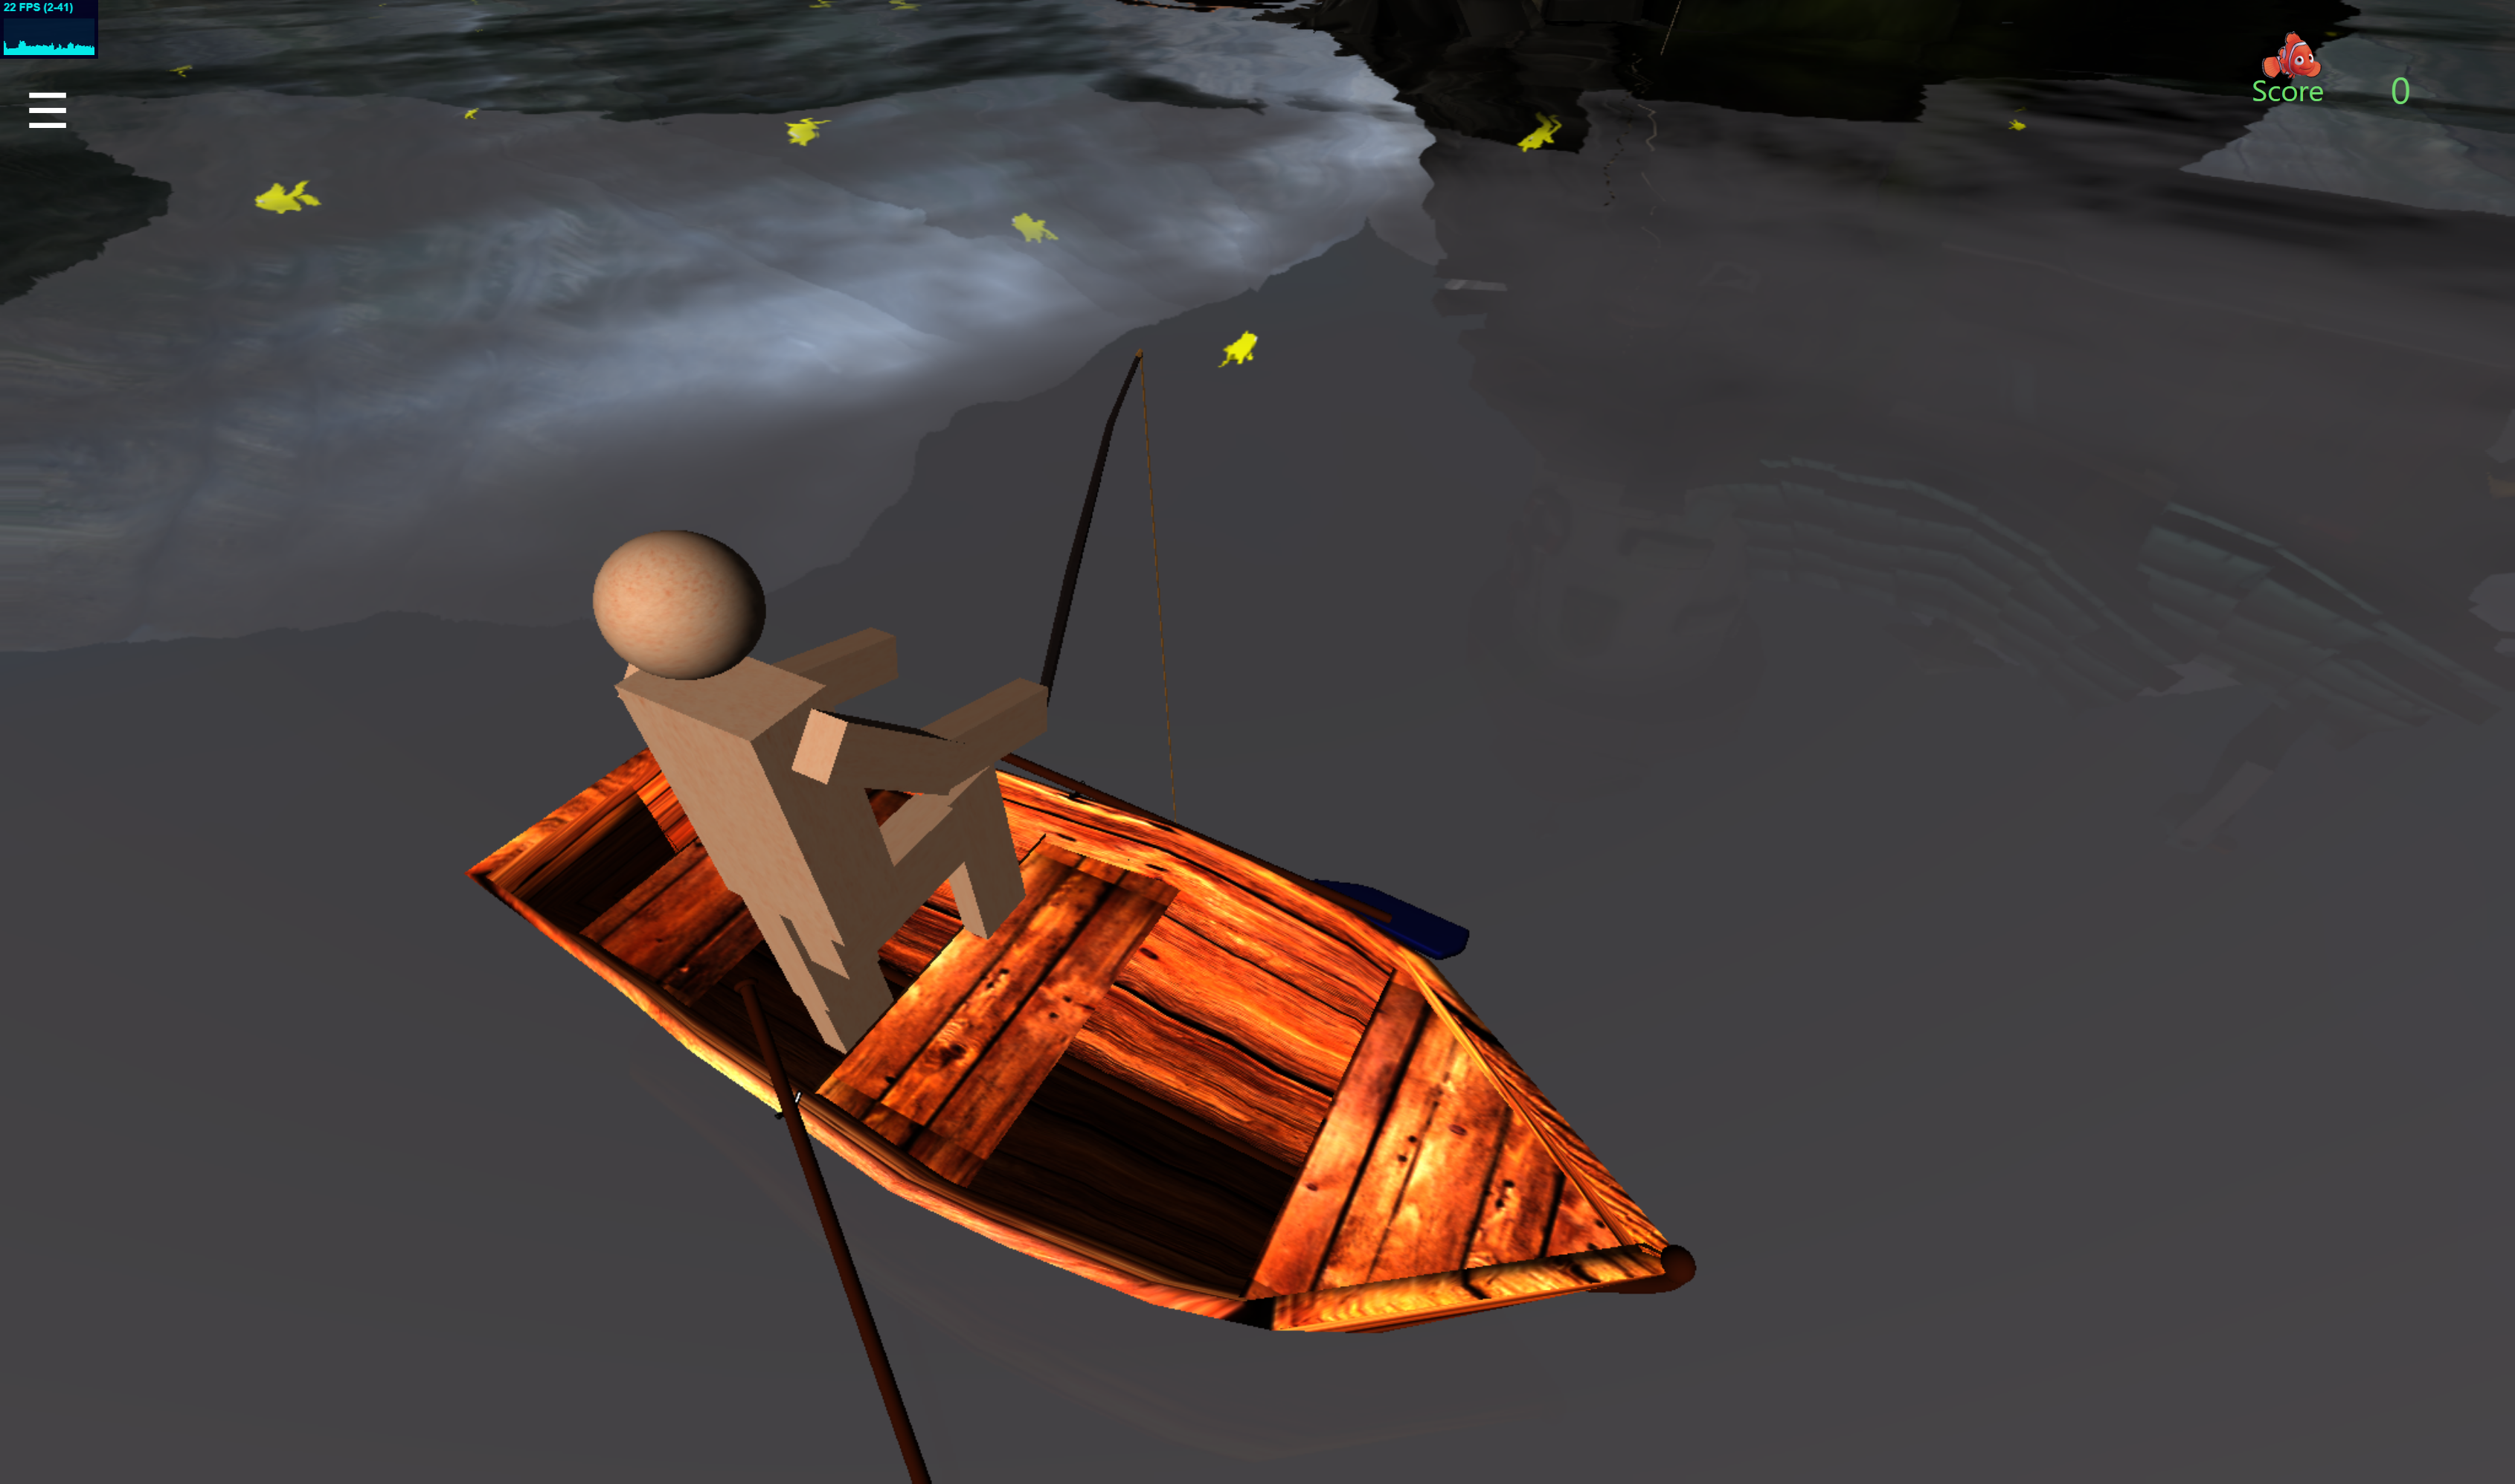
\includegraphics[width=15cm, height=7cm]{images/fishing_mode.png}
\caption{Camera view in fishing mode}
\label{fishing view}
\end{figure}

\begin{figure}[!ht]
\centering
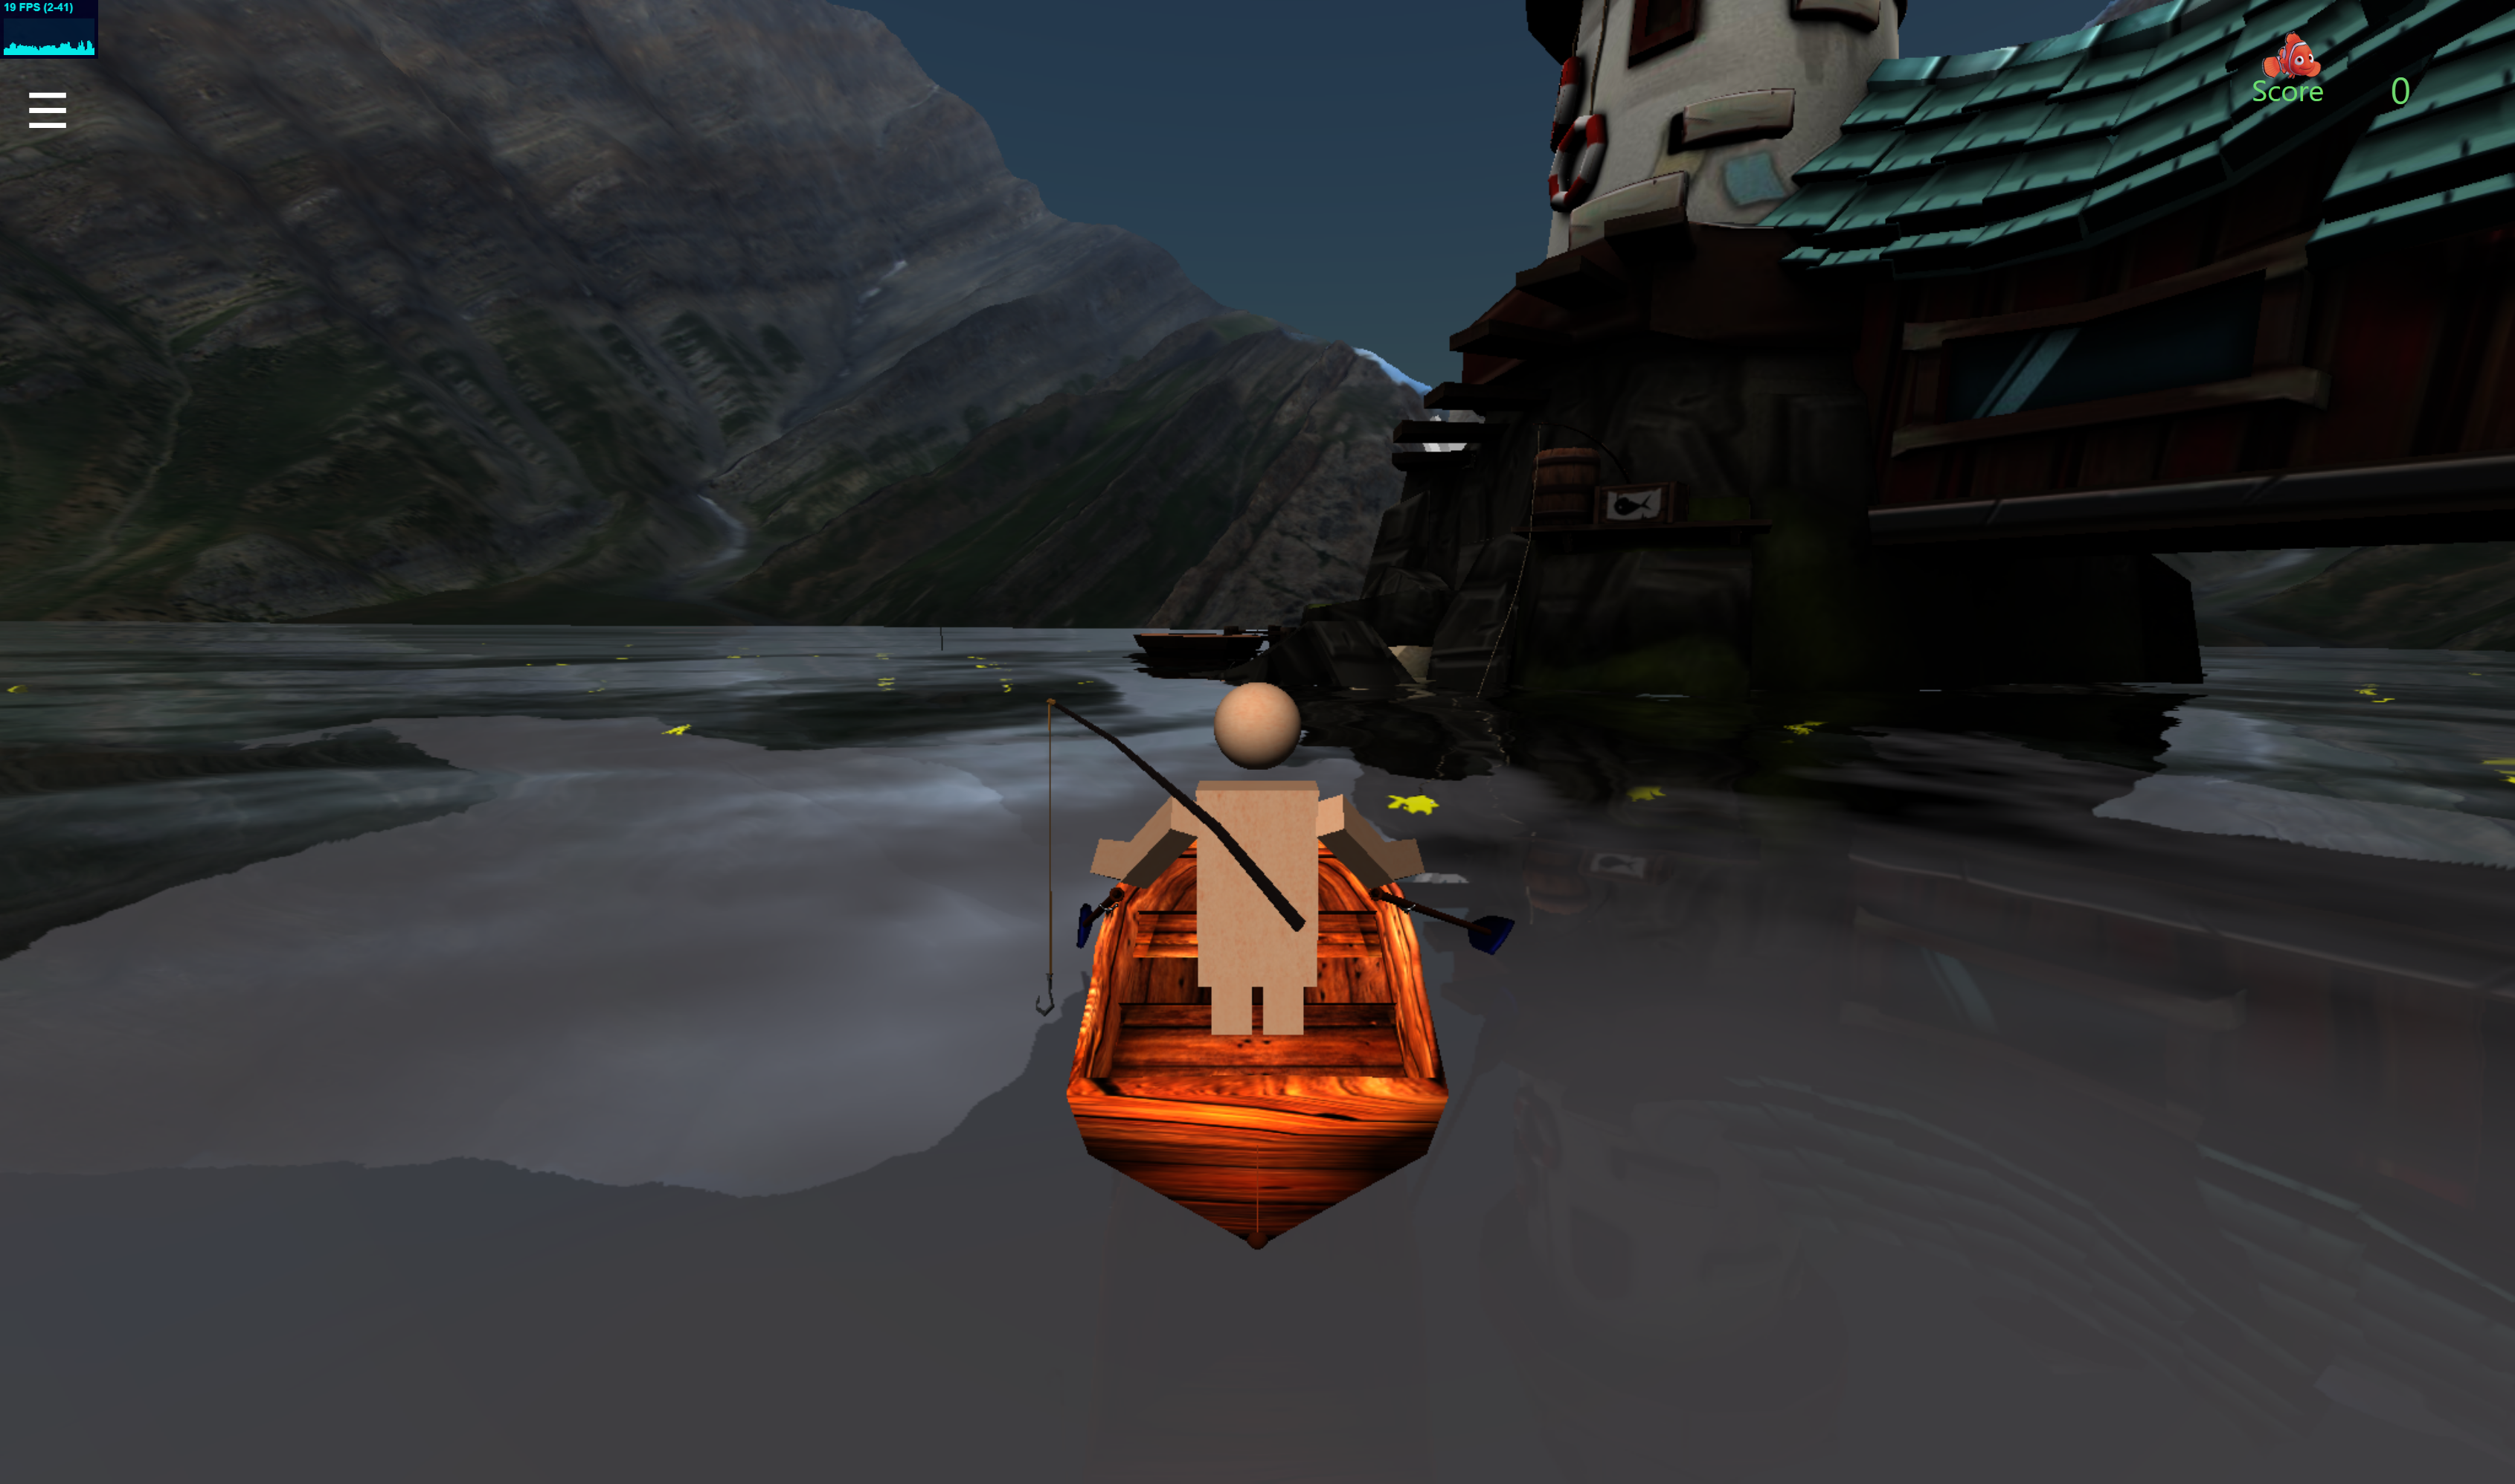
\includegraphics[width=15cm, height=7cm]{images/navigation_mode.png}
\caption{Camera view in navigation mode}
\label{navigation view}
\end{figure}
\newpage
\subsection{Fishes}

A 3D model of a goldfish was imported and used, it was added to the scene a Hundred times, each with a different name. The fishes move randomly in the environment at a constant speed. They move randomly, in order to make it more difficult for the user to predict the next direction of the fish, which makes the game harder and the collision more difficult to happen. The fishes were put at a depth of 20 pixels below the water surface (see \ref{fishes}), which is their fixed depth. 

\begin{figure}[!ht]
\centering
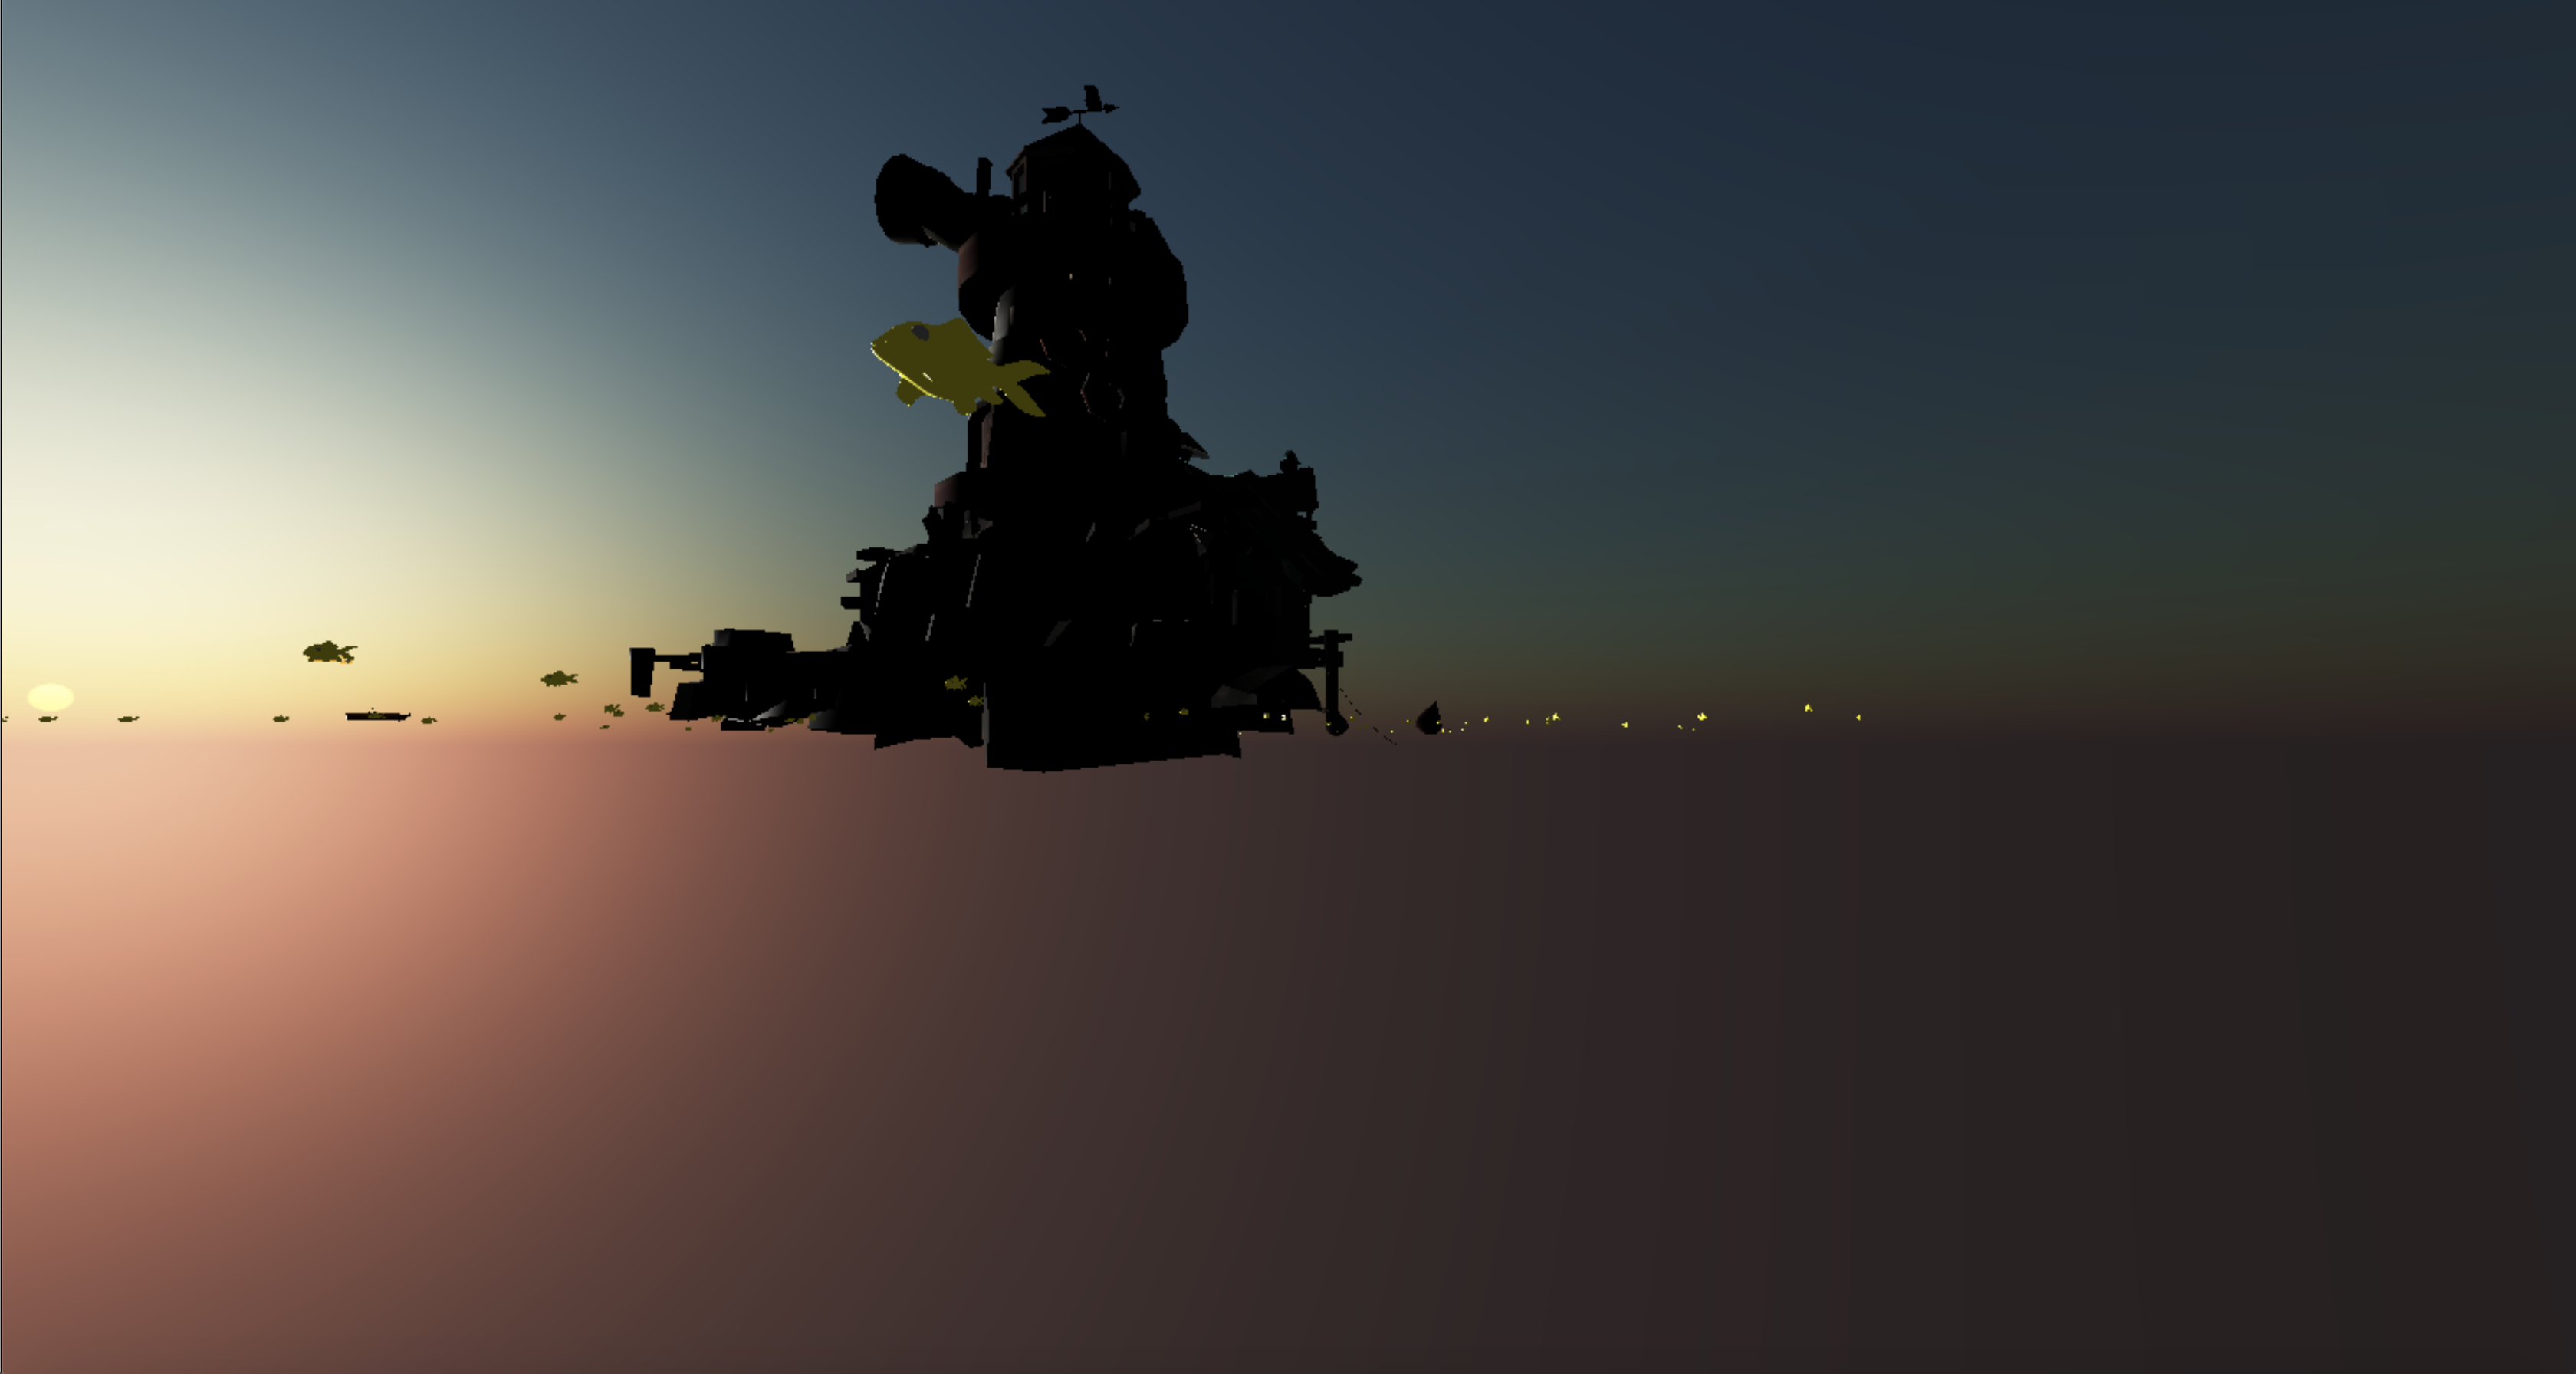
\includegraphics[width=15cm, height=7cm]{images/fishes.png}
\caption{Fishes view from underneath the water.}
\label{fishes}
\end{figure}
\newpage
\subsection{Collision}

In order for a collision between the bait and a fish to happen, the bait and the fish should be covered by \textit{Boxes}. This can be achieved by creating boxes using the three.js box geometry. The fish and the bait should be at the same height on the Y axis, which is 20 pixels below the water surface as previously stated. The vertical axis here is Y, since we are using three.js and this is the reference frame orientation in this library. They also should be on the same X, and Z axes points. Boxes were created and coded so as to follow the fishes and the bait movements, so a collision happens when wires of 2 boxes intersect. 
\newline

\textbf{Boxes code}
\begin{minted}{js}
var box = new THREE.Box3().setFromObject(bait);
var cubeGeometry = new THREE.BoxGeometry(box.getSize(center).x, 
    box.getSize(center).y, box.getSize(center).z);
var wireMaterial = new THREE.MeshBasicMaterial({
    opacity: 0,
    color: 0xFFFFFF,
    wireframe: true
});
baitBox = new THREE.Mesh(cubeGeometry, wireMaterial);
scene.add(baitBox);
\end{minted}
\par

\newpage
\section{Conclusions}
Finally, a \textit{Homepage} containing the information about the game and its developers has been added at the beginning of the game. A controls menu was also created containing the control keys that can be used to play the game. Moreover, an FPS counter, in the top right of the page, due to the heavy load of the game. Also background and events audio sounds, were coded and inserted into the game, such as a relaxed whistling or the cast and pull up sounds.

\subsection{Launching The Game}
For the application to run, we need first to establish a local server, which can be done using python through navigating to the game's directory using the command prompt (terminal shell) and writing: "python -m http.server". After the connection is established, one can open a browser and type "localhost:8000", this will allow the game to load in the browser page.

\section{Future Improvements}
\begin{itemize}
\item  Levelling System
\item Adding Physics to the Fishing Rod
\item Randomize Fish Size and Adjust the Score Based on That
\item With a certain Probability, Fishes are Moving to the Bait
\end{itemize}

\section{Libraries, Frameworks and References}
\textbf{Three.js} is a cross-browser JavaScript library, based on WebGL, and Application Programming Interface (API) used to create and display animated 3D computer graphics in a web browser.  The entire scene and all the libraries such as water, sky, camera controls and loader is made in Three.js
\\~\\
\textbf{Sketchfab} was used to download the raw 3D objects, such as the boat, rod, fishes, and lighthouse.
\\~\\
\textbf{Blender} was used to correct the the reference frames of the objects, the orientation and other minor adjustments


\end{document}\]
\end{document}